\documentclass[a4paper,12pt]{article}

\usepackage{float}


\usepackage[utf8]{inputenc}
\usepackage[dvips]{graphicx}
%\usepackage{a4wide}
\usepackage{epsfig}
\usepackage{fancybox}
\usepackage{verbatim}
\usepackage{array}
\usepackage{latexsym}
\usepackage{alltt}
\usepackage{amssymb}
\usepackage{amsmath,amsthm}
\usepackage{bm}
\usepackage{wasysym}

%\usepackage{fullpage}
%\usepackage{hyperref}
\usepackage{listings}
\usepackage{color}
\usepackage{algorithm}
\usepackage{algpseudocode}
\usepackage[hmargin=2cm,vmargin=3.0cm]{geometry}
%\topmargin=0cm
%\topmargin=-1.8cm
%\addtolength{\textheight}{6.5cm}
%\addtolength{\textwidth}{2.0cm}
%\setlength{\leftmargin}{-3cm}
%\setlength{\oddsidemargin}{0.0cm}
%\setlength{\evensidemargin}{0.0cm}

%misc libraries goes here
\usepackage{tikz}
\usepackage{tikz-qtree}
\usetikzlibrary{automata,positioning}

\usepackage{multicol}
\usepackage{enumitem}

\usepackage[most]{tcolorbox}

\usepackage[colorlinks=true,urlcolor=black,linkcolor=black]{hyperref}


\lstdefinestyle{customtex}{
    %backgroundcolor=\color{lbcolor},
    tabsize=2,
    language=TeX,
    numbers=none,
    basicstyle=\footnotesize\ttfamily,
    numberstyle=\footnotesize,
    aboveskip={0.0\baselineskip},
    belowskip={0.0\baselineskip},
    %
    columns=flexible,
    keepspaces=true,
    fontadjust=true,
    upquote=true,
    %
    breaklines=true,
    prebreak=\raisebox{0ex}[0ex][0ex]{\ensuremath{\hookleftarrow}},
    frame=single,
    showtabs=false,
    showspaces=false,
    showstringspaces=false,
    %
    %identifierstyle=\color[rgb]{0,0.2,0.8},
    identifierstyle=\color[rgb]{0,0,0.5},
    %identifierstyle=\color[rgb]{0.133,0.545,0.133},
    %keywordstyle=\color[rgb]{0.8,0,0},
    %keywordstyle=\color[rgb]{0.133,0.545,0.133},
    keywordstyle=\color[rgb]{0,0,0.5},
    %commentstyle=\color[rgb]{0.133,0.545,0.133},
    commentstyle=\color[rgb]{0.545,0.545,0.545},
    %stringstyle=\color[rgb]{0.827,0.627,0.133},
    stringstyle=\color[rgb]{0.133,0.545,0.133},
    %
    literate={â}{{\^{a}}}1 {Â}{{\^{A}}}1 {ç}{{\c{c}}}1 {Ç}{{\c{C}}}1 {ğ}{{\u{g}}}1 {Ğ}{{\u{G}}}1 {ı}{{\i}}1 {İ}{{\.{I}}}1   {ö}{{\"o}}1 {Ö}{{\"O}}1 {ş}{{\c{s}}}1 {Ş}{{\c{S}}}1 {ü}{{\"u}}1 {Ü}{{\"U}}1 {~}{$\sim$}{1}
}

\lstdefinestyle{output}{
    %backgroundcolor=\color{lbcolor},
    tabsize=2,
    numbers=none,
    basicstyle=\footnotesize\ttfamily,
    numberstyle=\footnotesize,
    aboveskip={0.0\baselineskip},
    belowskip={0.0\baselineskip},
    %
    columns=flexible,
    keepspaces=true,
    fontadjust=true,
    upquote=true,
    %
    breaklines=true,
    prebreak=\raisebox{0ex}[0ex][0ex]{\ensuremath{\hookleftarrow}},
    frame=single,
    showtabs=false,
    showspaces=false,
    showstringspaces=false,
    %
    %identifierstyle=\color[rgb]{0.44,0.12,0.1},
    identifierstyle=\color[rgb]{0,0,0},
    keywordstyle=\color[rgb]{0,0,0},
    commentstyle=\color[rgb]{0,0,0},
    stringstyle=\color[rgb]{0,0,0},
    %
    literate={â}{{\^{a}}}1 {Â}{{\^{A}}}1 {ç}{{\c{c}}}1 {Ç}{{\c{C}}}1 {ğ}{{\u{g}}}1 {Ğ}{{\u{G}}}1 {ı}{{\i}}1 {İ}{{\.{I}}}1   {ö}{{\"o}}1 {Ö}{{\"O}}1 {ş}{{\c{s}}}1 {Ş}{{\c{S}}}1 {ü}{{\"u}}1 {Ü}{{\"U}}1
}

\lstset{style=customtex}


\tikzset{%
    terminal/.style={draw, rectangle,
    				 align=center, 
					 minimum height=1cm, 
					 minimum width=2cm,
					 fill=black!10,
					 anchor=mid},
    nonterminal/.style={draw, rectangle,
    					align=left,
					    minimum height=1cm, 
						minimum width=2cm, 
						anchor=mid},% and so on
}

%% Style for terminals
%\tikzstyle{terminal}=[draw, rectangle, 
%					  minimum height=1cm, 
%					  minimum width=2cm, 
%					  fill=black!20,
%					  anchor=south west]
%% Style for nonterminals
%\tikzstyle{nonterminal}=[draw, rectangle, 
%						 minimum height=1 cm, 
%						 minimum width=2 cm, 
%						 anchor=north east]


\newcommand{\HRule}{\rule{\linewidth}{1mm}}
\newcommand{\kutu}[2]{\framebox[#1mm]{\rule[-2mm]{0mm}{#2mm}}}
\newcommand{\gap}{ \\[1mm] }

\newcommand{\Q}{\raisebox{1.7pt}{$\scriptstyle\bigcirc$}}
\newcommand{\minus}{\scalebox{0.35}[1.0]{$-$}}

\setlength{\fboxsep}{10pt}

\tcbsetforeverylayer{enhanced jigsaw, breakable, arc=0mm, boxrule=1pt, boxsep=5pt, after=\vspace{1em}, colback=white, colframe=black}

\newcolumntype{P}[1]{>{\centering\arraybackslash}p{#1}}

\setlength\parindent{0pt}

%\renewcommand\arraystretch{1.2}

\newenvironment{Tab}[1]
  {\def\arraystretch{1}\tabular{#1}}
  {\endtabular}

%%%%%%%%%%%%%%%%%%%%%%%%%%%%%%%%%%%%%%%%%%%%%%%%%%%%%%%%%%%%%%%%%%%%%%%%%%%%%%%%%%%%%%

\title{CENG 352 - Database Management Systems \\ Written Assignment 2}
\author{Alper KOCAMAN \\ 2169589} % write your name and id
\date{05.04.2020}

%%%%%%%%%%%%%%%%%%%%%%%%%%%%%%%%%%%%%%%%%%%%%%%%%%%%%%%%%%%%%%%%%%%%%%%%%%%%%%%%%%%%%%

\begin{document}
\HRule\\
Middle East Technical University \hfill Department of Computer Engineering
{\let\newpage\relax\maketitle}
\HRule\\
\vspace{1cm}

%%%%%%%%%%%%%%%%%%%%%%%%%%%%%%%%%%%%%%%%%%%%%%%%%%%%%%%%%%%%%%%%%%%%%%%%%%%%%%%%%%%%%%

% Write your answers below the section tags
\section{ \hfill}

\paragraph{a)} Yes, the query in the Q1.a can be evaluated by the index only plan. \\ We have a condition on "age" column. After getting the appropriate records, we need to form groups according to records' "age" column. All these operations can be done in the index structure and no record is needed to be fetched from the secondary storage. Furthermore, we can count the records for each "age" group from the index. Also, since "select" statement does not contain a column that is not in the index, we can execute this query only from the index.\\  

\paragraph{b)} No, the query in the Q1.b cannot be evaluated by the index only plan. \\ The index structure has a composite search key on (age,grade). This means that built index structure is aware of "age" and "grade" columns. However, there is a "gender" information needed in the "where" clause of the query. In order this query to be executed, the related records must be fetched from the secondary storage, index structure is not sufficient to execute this query. 

\newpage

\section{}

\paragraph{a)}  $\sigma_A=500.000$

\begin{tcolorbox}
Usage of heap file(pile file) will be inefficient since we need to look lots of records in order to find the requested one.(needs lots of I/O operations) \\
Usage of unclustered B+ tree index will be efficient since we can find the requested record by just tracing a couple of pointers in tree nodes.(needs only 1 I/O operation) \\
Usage of clustered B+ tree will also have a very little cost like unclustered B+ tree.(needs only 1 I/O operation) \\
Usage of hash index will be very efficient because we can get the record by just following the output of the hash function.(needs only 1 I/O operation)\\
Thus, all given methods will be useful in this case except heap file option.
\end{tcolorbox}

\paragraph{b)}$\sigma_A<20.000$

\begin{tcolorbox}
Usage of heap file(pile file) will be very inefficient since we need to look lots of records in order to find the records which have a value less than $20.000$ in their A attribute.\\
Usage of unclustered B+ tree index will be inefficient as well.Although we can find the requested range by using index, the data resides in a distributed way in the secondary storage.This means that lots of I/O operation might be needed to get the records. \\
Usage of clustered B+ tree will be best in this kind of queries. We can find the requested range by using index. Since the file is sorted on the A attribute in the secondary storage, when a page fetched from there, lots of other records that fall into the same range are also fetched. Thanks to this mechanism, number of I/O operation needed is really less in clustered B+ tree compared to the other methods.\\
Usage of hash index will not be logical because hash indexes are not useful for range queries.\\
Thus, usage of clustered B+ tree index will be expected to have least cost.
\end{tcolorbox}

\paragraph{c)}$\sigma_A>20.000 \wedge \sigma_A<20.010$

\begin{tcolorbox}
Usage of heap file(pile file) will be very inefficient since we need to examine lots of needless records in order to find the actual ones.\\
Usage of unclustered B+ tree index might be inefficient as well since the data might be distributed in the secondary storage.This method will need 10 I/O operation in order to get the result set in the worst case scenario. However, 10 I/O operations is not a huge job for computers nowadays and  this method will be acceptable. \\
Usage of clustered B+ tree will be best again. We can find the requested range by just using B+ index. Since the file is sorted on the A attribute and one data page can hold 10 records , we can fetch the results in just 1 I/O operation.\\
Again, usage of hash index will not be efficient because hash indexes are not useful for range queries. However, requested records number is 10(relatively small number) and this method will be acceptable as well. \\
Thus, usage of clustered B+ tree index will be best(only 1 I/O operation is needed).\\
Unclustered B+ tree and hash index methods will not serve a better performance than clustered B+ tree, but they are acceptable as well.
\end{tcolorbox}

\paragraph{d)}$\sigma_A\neq 500.000$

\begin{tcolorbox}
Usage of unsorted heap file will fetch all the pages. This means that $1.000.000$ pages should be retrieved. Also, finding the record which has a A value as $500.000$ will add an additional cost.\\
Usage of unclustered B+ tree will retrieve results tuple by tuple. A page is fetched and one of the 10 record is extracted. In this method, one record may be fetched more than once, and this adds a overhead inevitably.\\
Usage of clustered B+ tree will need to fetch all pages as well. Unlike unclustered B+ tree, clustered B+ tree will not retrieve the same record more than once since records are sorted on A. Tree lookup process may add an additional cost in this case.\\
Using hash index might not be a good idea because it performs like unclustered B tree in this case. One page may be fetched more than once.\\
Thus, usage of pile file or clustered B+ tree work best on this query. I expect that their performance are nearly equivalent.
\end{tcolorbox}

\newpage

\section{}

\paragraph{a)} Equivalent logical query plan of the query in Q3.a : 

\begin{figure} [H]
    \centering
    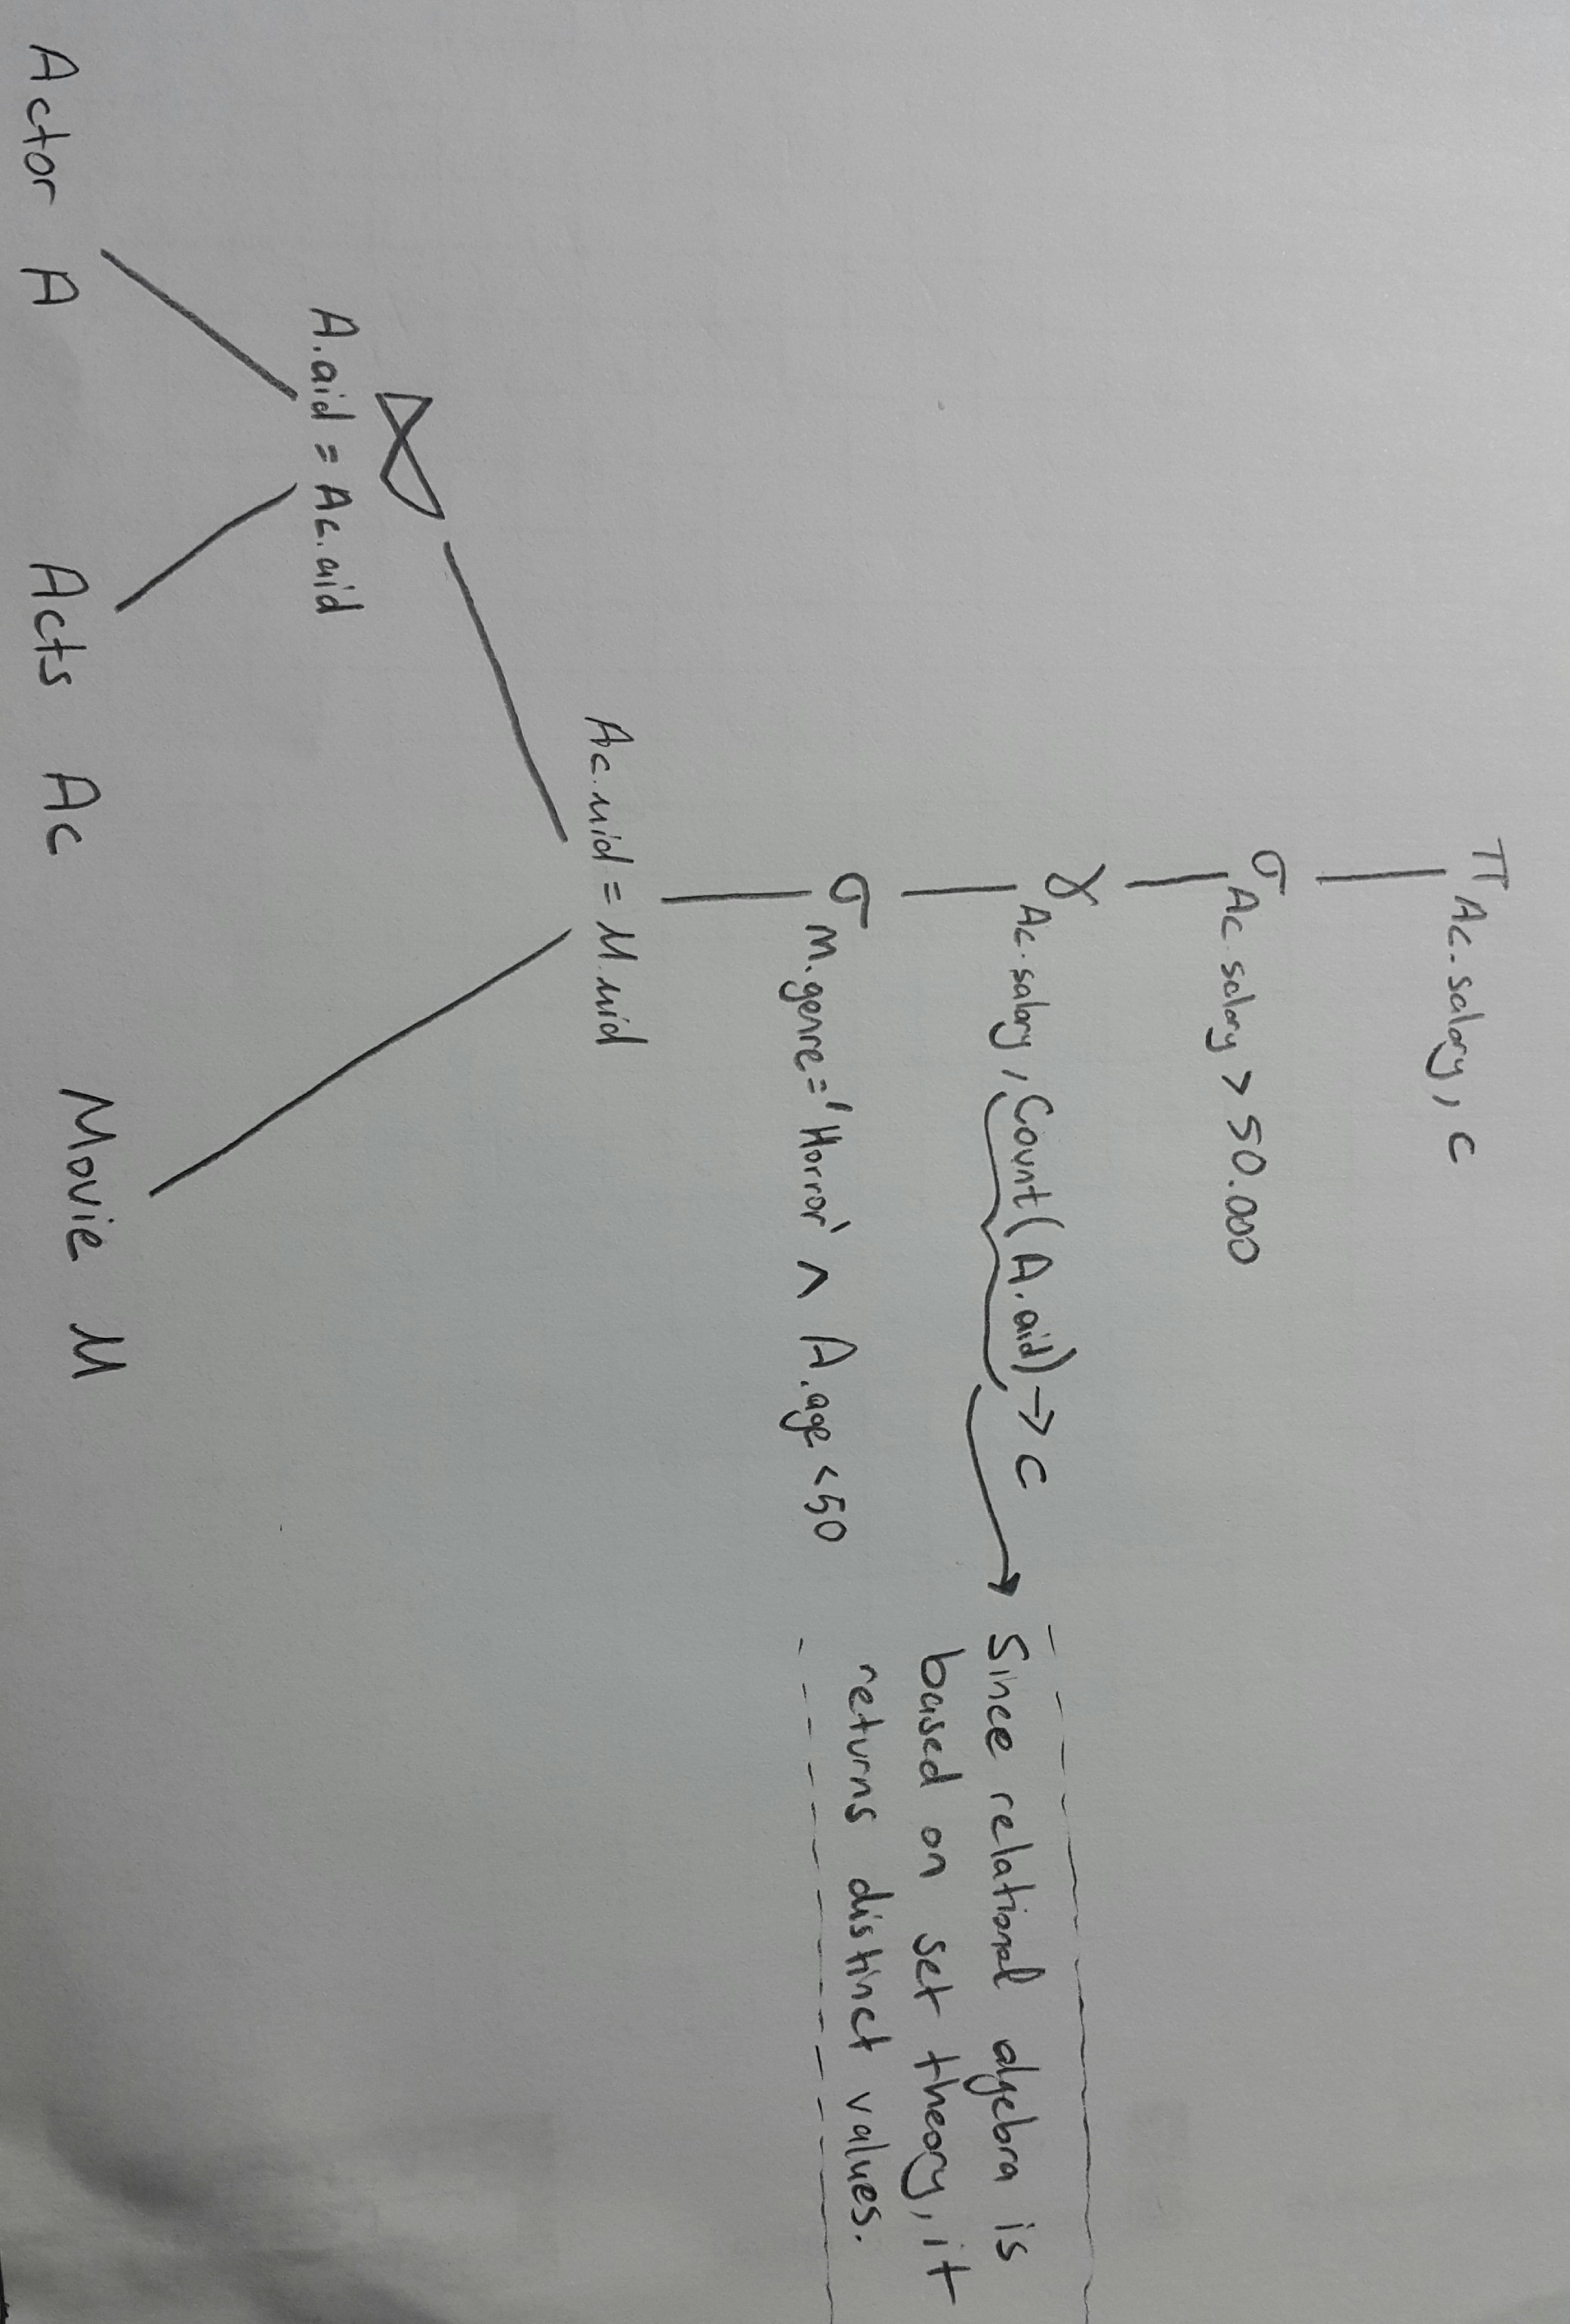
\includegraphics[scale=0.2]{3.a.jpg}
\end{figure}

\paragraph{b)} Equivalent logical query plan of the query in Q3.b : \\

\begin{figure} [H]
    \centering
    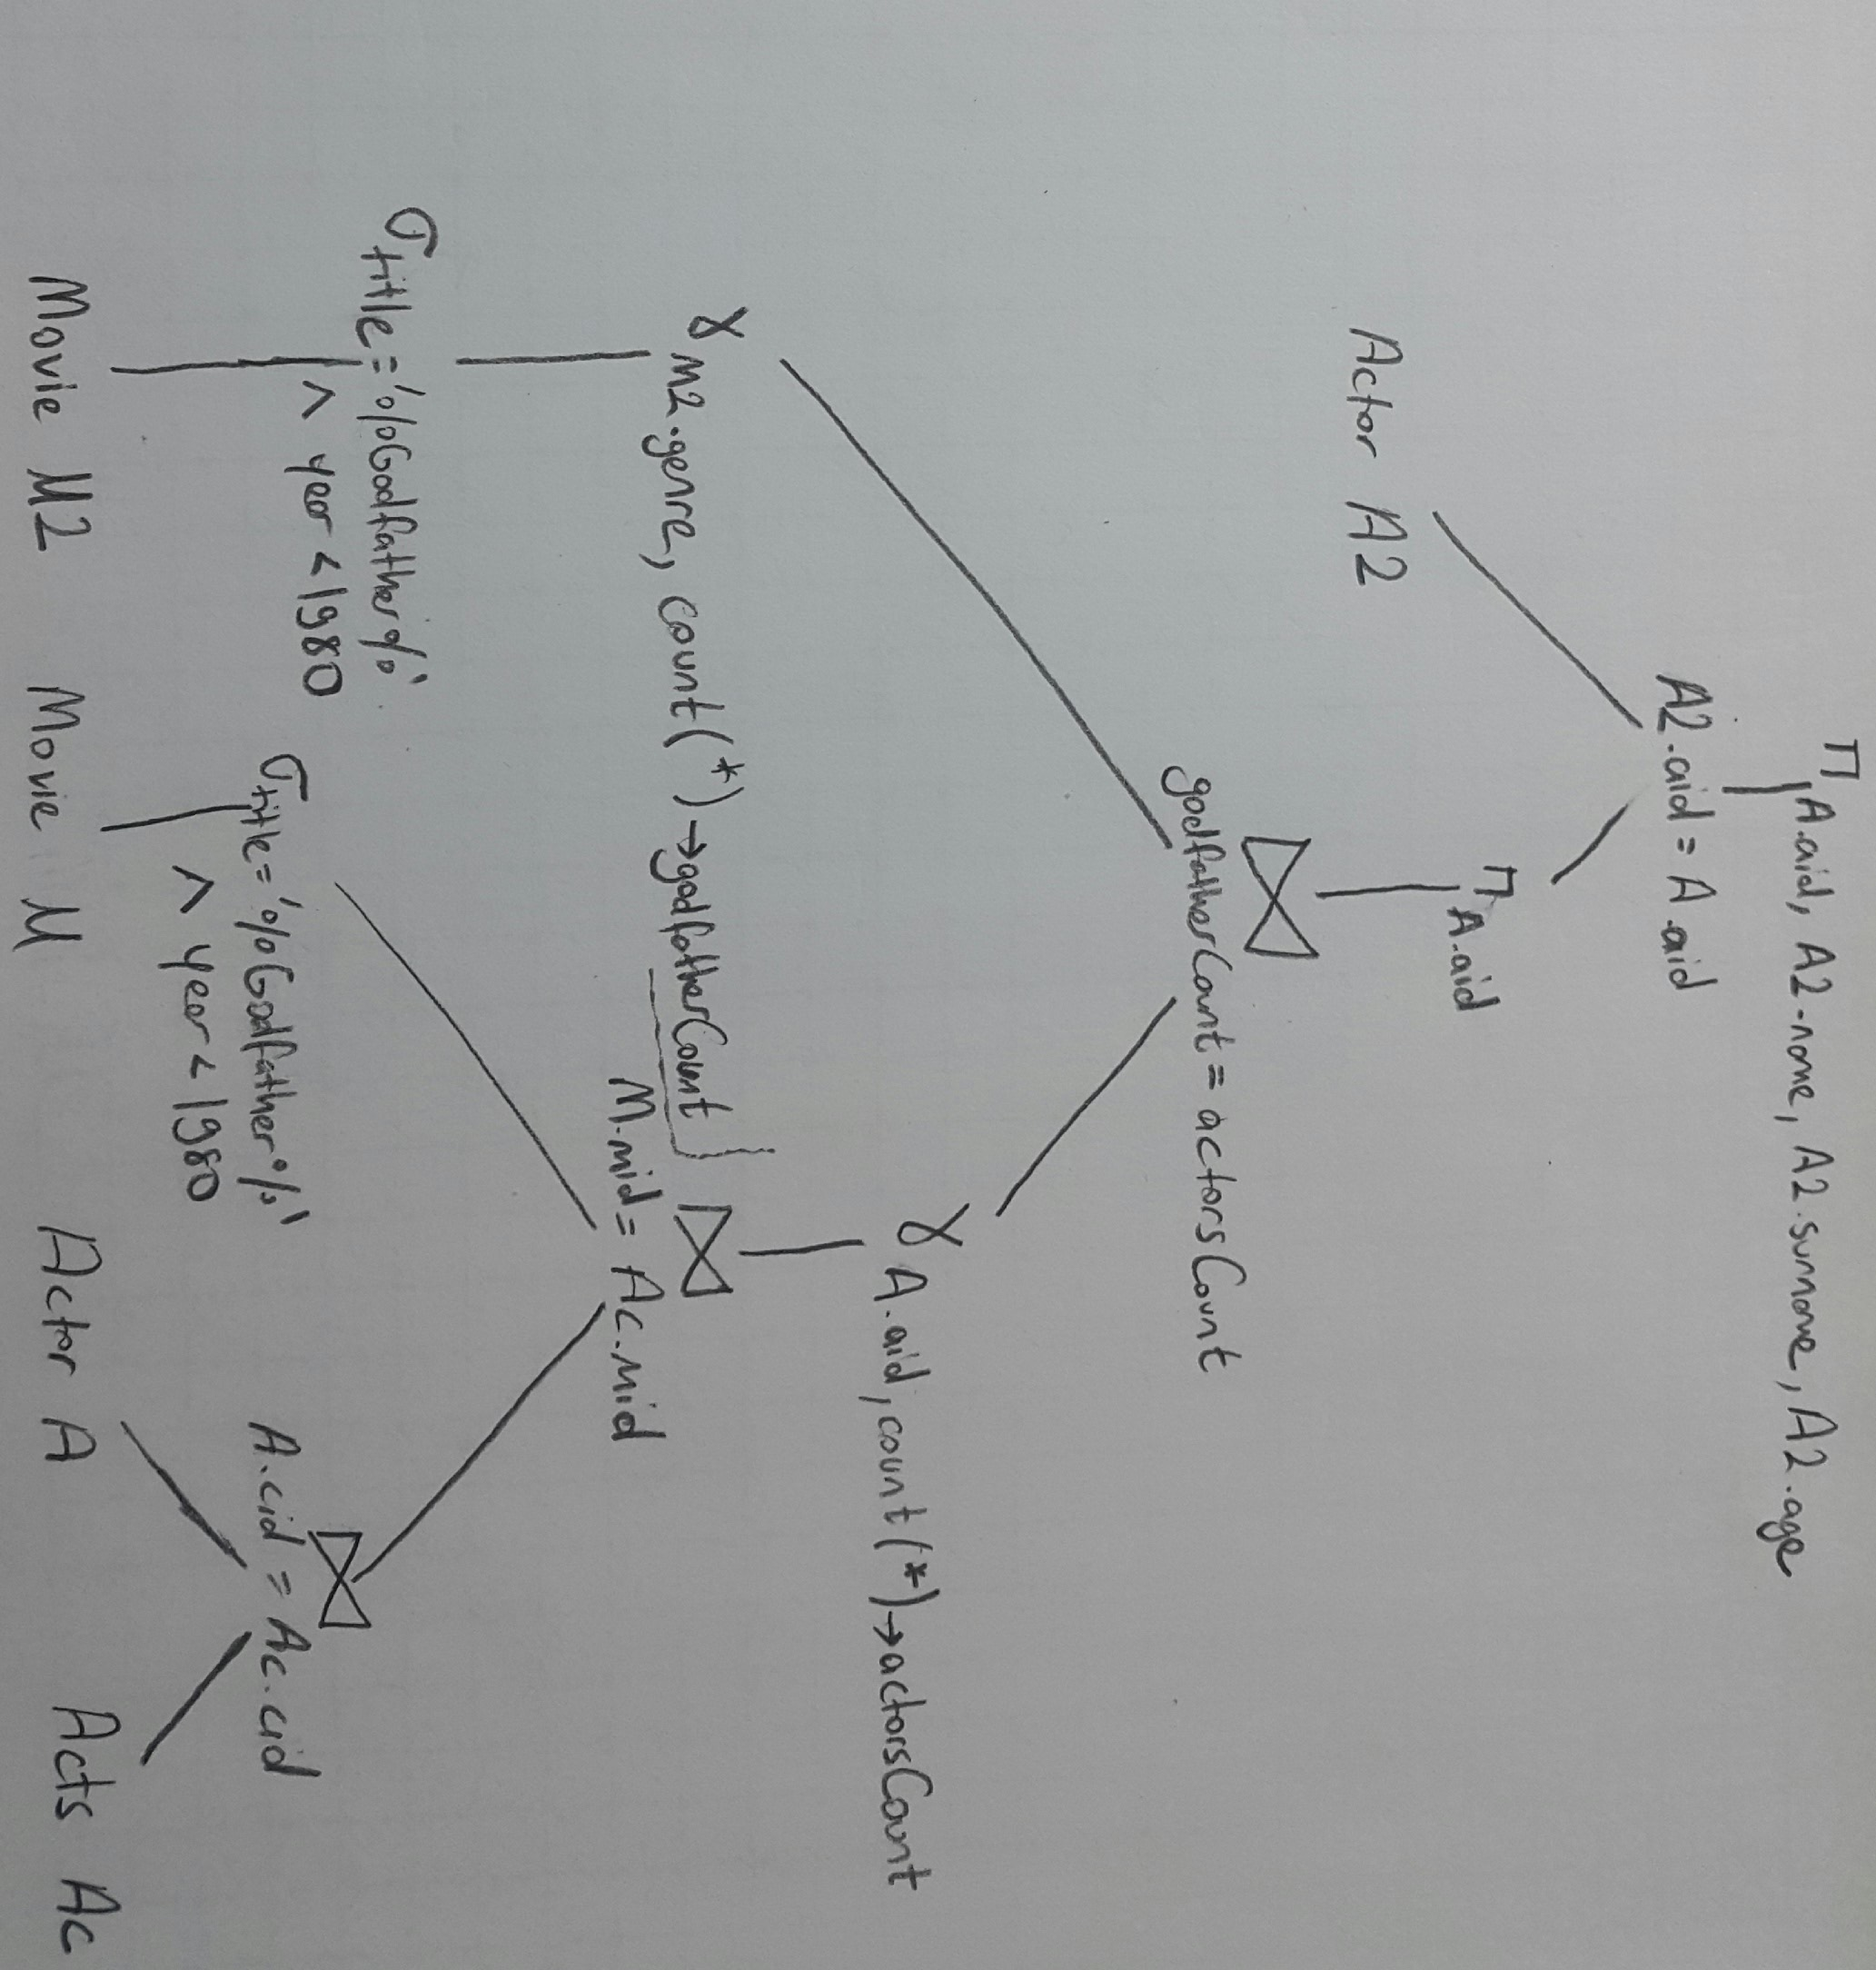
\includegraphics[width=\linewidth]{3.b.jpg}
\end{figure}
\newpage

\section{}

\paragraph{a)} 
Cost of joining R and S using a block nested loops join when R is the outer relation
\begin{tcolorbox}
$B(R) = T(R)/$tuple per page $\rightarrow$ $B(R) = T(R)/10$ $\rightarrow$ $B(R) = 20.000/10\ = 2000$. \\
$B(S) = T(S)/$tuple per page $\rightarrow$ $B(S) = T(S)/10$ $\rightarrow$ $B(S) = 5.000/10\ = 500$.\\
Number of available buffer pages $M = 42$.\\
Since cost function of the block nested loops join is $\frac{B(R)\times B(S)}{M-2} + B(R)$,\\ resulting cost is $2000+\frac{2000\times 500}{40} =\ 27000$. 
\end{tcolorbox}

\paragraph{b)}  
Cost of joining R and S using a block nested loops join when S is the outer relation
\begin{tcolorbox}
$B(R) = T(R)/$tuple per page $\rightarrow$ $B(R) = T(R)/10$ $\rightarrow$ $B(R) = 20.000/10\ = 2000$. \\
$B(S) = T(S)/$tuple per page $\rightarrow$ $B(S) = T(S)/10$ $\rightarrow$ $B(S) = 5.000/10\ = 500$.\\
Number of available buffer pages $M = 42$.\\
Since cost function of the block nested loops join is $\frac{B(R)\times B(S)}{M-2} + B(S)$,\\ resulting cost is $500+\frac{2000\times 500}{40} =\ 25500$.
\end{tcolorbox}

\paragraph{c)} 

\begin{tcolorbox}
$B(R) = T(R)/$tuple per page $\rightarrow$ $B(R) = T(R)/10$ $\rightarrow$ $B(R) = 20.000/10\ = 2000$. \\
$B(S) = T(S)/$tuple per page $\rightarrow$ $B(S) = T(S)/10$ $\rightarrow$ $B(S) = 5.000/10\ = 500$.\\
If we want to use 2 pass sort-merge join, the following condition should be met:\\
$M^2 \geq B(R)$ $\rightarrow$ $42^2 \geq 2000$ which does not hold. Thus, we cannot apply 2 pass sort merge join in this case. We need more pass in this setup.\\
We need to generate runs for both relation R and relation S. Initially, relation R is read from the secondary storage, sorted in the memory and written to the disk. Then, relation S is read from the secondary storage, sorted in the memory and written to the disk. In these processes, all 42 pages are used.At the end,\\
$2000/42 = 47.61$ which is 48(because of ceiling function) runs of R and,\\
$500/42 = 11.90$ which is 12(because of ceiling function) runs of S are formed.\\ 
These processes cost is $2B(R)+2B(S)$.\\
Since page number is 42 and total runs number is $48+12=60$, we cannot merge them directly. Runs of relation R should be merged firstly. We can create 2 chunks of R by using 1 page in the memory as output page and 41 pages in the memory for sorted pages of it.\\
At the end of this step, since we read the whole R sorted runs to memory and after merging, since we write it again to the secondary disk, cost of these processes are $B(R)+B(R) = 2B(R)$.\\
Then, we have 2 chunks for relation R and 12 runs for relation S. In the memory, 2 page is allocated for chunks of R, 12 pages are allocated for runs of S and 1 page is allocated for output. This merging process also costed as $B(R)+B(S)$ since we read them from the secondary disk.\\
After these steps, we have joined relation R and relation S by using sort-merge join.\\
Costs of operations were mentioned while operations were being explained.\\ When we add up them,\\
$2B(R)+2B(S)+2B(R)+B(R)+B(S)\ =\ 5B(R)+3B(S)\ =\ 5\times 2000+ 3\times 500\ =\ 11500$. 

\end{tcolorbox}

\paragraph{d)}

\begin{tcolorbox}
$B(R) = T(R)/$tuple per page $\rightarrow$ $B(R) = T(R)/10$ $\rightarrow$ $B(R) = 20.000/10\ = 2000$. \\
$B(S) = T(S)/$tuple per page $\rightarrow$ $B(S) = T(S)/10$ $\rightarrow$ $B(S) = 5.000/10\ = 500$.\\
Firstly,in order to apply hash join, the following condition should be met:\\
$min(B(R),B(S))\leq M^2$ $\rightarrow$ $min(2000,500)\leq 42^2$ $\rightarrow$ $500\leq 1764$.\\
Since the condition is met, hash join with 2 pass can be applicable.\\
In order to apply partitioned hash join, we need to create hashes of both relation R and relation S.\\
Firslty, we need to read relation S one page at a time and hash them into $M-1=41$ buckets.In this step, when a bucket fills up, it is flushed into the disk.At the end, we get relation S on disk splitted into 41 buckets.\\
After getting hashes of S, we need to read relation R one page at a time and hash them into $M-1=41$ buckets again.Like in relation S, when a bucket fills up in the memory, it is flushed into the disk.At the end, we also get relation R on disk splitted into 41 buckets.\\
Then, algorithm reads one partition of R and create hash table in memory using a different hash function. In this step, 1 page is separated for input buffer, 1 page is separated for output buffer and 40 pages are available for hash table.\\
After than,we should scan matching partition of S by using hash table. When this process is repeated for all buckets, partitioned hash join ends.\\ 
Total cost of this 2 pass hash join formula is $3B(R) + 3B(S)$,\\
$3\times 2000 + 3 \times 500 = 7500$
I/Os.
\end{tcolorbox}

\paragraph{e)}

\begin{tcolorbox}
$B(R) = T(R)/$tuple per page $\rightarrow$ $B(R) = T(R)/10$ $\rightarrow$ $B(R) = 20.000/10\ = 2000$. \\
$B(S) = T(S)/$tuple per page $\rightarrow$ $B(S) = T(S)/10$ $\rightarrow$ $B(S) = 5.000/10\ = 500$.\\
We need to find corresponding relation S tuples for all tuples of relation R in order to join these two relations.\\
For clustered index, we can trace the pointers in the B+ tree node and find the actual place in the secondary storage. Likewise, in unclustered index, we can work by tracing the pointers in the tree nodes. When we get a page from a clustered index, we get similar records with it since records are sorted. Their difference is that in an unclustered index, possibility of the page miss is much higher.\\
However, we need to notice one thing in question, we are joining R relation with S relation by using S.b attribute which is a primary key. Thus, we can expect equivalent cost.\\
Unclustered index cost = $B(R)+\frac{T(R)\times T(S)}{V(S,b)}$ $\rightarrow$ $2.000+\frac{20.000*5000}{5000}\ =\ 22.000$.\\  
Normally, clustered index cost formula is \\$B(R)+\frac{T(R)\times B(S)}{V(S,b)}$.\\ However, since S.b attribute is primary key, we need to select all tuples again. Thus, B(S)/V ratio in the formula becomes 1.\\ Total cost for clustered index is again $2.000+20.000*1\ =\ 22.000$.\\

\end{tcolorbox}

\newpage
\section{}

\paragraph{a)}

\begin{tcolorbox}
The total number of all clothing items that are sold in the m10, m11 and m12 can be found by adding them.($m10+m11+m12$).\\
Ratio of the swimsuits in whole clothing items can be found by dividing swimsuit number to all clothing items.($\frac{t_{swim}}{N}$).\\
When we multiply these obtained expressions, we get the estimate of the swimsuit number that are sold in the 10,11 and 12. months.\\
Answer is $\frac{t_{swim}\times (m10+m11+m12)}{N}$.
\end{tcolorbox}

\paragraph{b)}

\begin{tcolorbox}
We assume that the clothes sold are distributed to year uniformly. Then, we solved the question by taking ratio of specific clothing to all clothes. However, this is not the case all the time.\\
In the example, we found the swim clothes. However, in the 10,11 and 12. months, we do not expect that swim clothes are sold.(If you are not living in the south hemisphere :))\\
Thus, this estimate is probably incorrect.
\end{tcolorbox}
\end{document}
